% TODO: Update this for proper formatting:
%\documentclass[12pt,times]{article}
\documentclass[12pt]{article} % \usepackage{times}
%\usepackage[a4paper, showframe, tmargin=25mm, lmargin=25mm, rmargin=25mm, bmargin=20mm]{geometry}
\usepackage[a4paper, tmargin=25mm, lmargin=20mm, rmargin=20mm, bmargin=20mm]{geometry}
\usepackage{amsmath,amssymb,amsthm}
\usepackage{color}
\usepackage{hyperref}
\usepackage{graphicx}
\usepackage{stmaryrd}
\usepackage{listings}
\usepackage{color}
\usepackage{wrapfig}
\usepackage{url}
\usepackage{fancyvrb}
\usepackage{placeins}
\usepackage{bold-extra}
\usepackage[nounderscore]{syntax}
\usepackage{mathtools}
\usepackage{caption}
\usepackage{float}

\usepackage{xcolor}
\usepackage{soul}

\usepackage{fancyhdr}
\pagestyle{fancy}
\rhead{Version: \GUIDEVERSION} 
\lhead{\GUIDETITLE}
%\cfoot{}
\thispagestyle{fancy}
% \thispagestyle{headings}

\newcommand{\GUIDEVERSION}[0]{$0.1$}
\newcommand{\GUIDETITLE}[0]{Tutorial: Add Functionality to the Demo Platform}

\newcommand{\change}[0]{\noindent{\hl {\b CODE CHANGE:}}}

\begin{document}

\title{\GUIDETITLE}


\author{The RISE Demo Platform Team}



\date{Version \GUIDEVERSION{} \today}




%  Use the @ symbol for simple inline code within prose:
\lstMakeShortInline[]@


\maketitle


\section{Introduction}

This document will take you through the procedure of adding some
functionality to the RC car demo platform. The functionality that is
added is a motor controller simulator that will allow us to use the RC
car controller board without a motor controller board connected. This
can be useful for simulation and experimentation without access to the
entire car setup (easy-access table-top experimentation).

Adding this functionality will take us through a number of files in both
the car GUI (for your linux device) {\verb!RControlStation!} and in the
embedded software running on the RC car controller. In total, changes
will be made to 15 files.

The purpose of this document is to serve as an introduction for
someone who has no familiarity with the software involved, a getting
started guide for the RC car software in other words.

Code presented in this document has often been abbreviated. This
is indicated by the comment {\verb!/* ... */!}. Some functions are
just too lengthy to include in full.

If you want to write the code yourself, either a direct copy of what is
presented here or your own, checkout using this command:

\begin{verbatim}
cd my_rise_sdvp_github_dir
git checkout df3dd9e32a7e78a24d1b5ce92d1b6cc78c3adba4
\end{verbatim}

This command transports you backwards in time, to before there was a
any motor simulation functionality on the demo platform. When doing the
work yourself, ignore all the text highlighted with ``\change{}'' and
skip section \ref{sec:implementation} (just peek at if you want a hint).
      
\section{Overview of Files to Edit} 

We will make changes both to RControlStation (The Qt based GUI) and to
the embedded software running on the RC car controller. We will begin
by adding a checkbox to the GUI and to do that we need to touch the
following RControlStation files:

\begin{itemize}
\item {\verb!Linux/RControlStation/datatypes.h!} \\ This file contains
  (amongst other things) the C struct used as the format for
  transferring data to and from the car. This struct is called
  {\verb!MAIN_CONFIG!} in the code.

  A field has to be added to this struct in order to communicate the
  state of the checkbox between the GUI and car.
  
\item {\verb!Linux/RControlStation/packetinterface.cpp!} \\ Controls
  the sending and receiving of, for example, the configuration data
  mentioned above over the packet interface. A small modification is
  needed here to facilitate the transfer of the state of the checkbox.
  
\item {\verb!Linux/RControlStation/carinterface.cpp!} \\ Contains the
  functions that bridge between the GUI and the data structures (for
  example the {\verb!MAIN_CONFIG!} struct). Here we need to add
  functions that update the {\verb!MAIN_CONFIG!} based on the state of
  the checkbox in the GUI.
\item {\verb!Linux/RControlStation/carinterface.ui!} \\
  This file is altered by Qt Creator when we edit the user interface to add the
  checkbox. We will not edit it manually. 
\end{itemize}

On the embedded end we will make alterations to the following files,
as well as adding two new files that are also listed here: 

\begin{itemize}
\item {\verb!Embedded/RC_Controller/datatypes.h!}  \\ Contains the
  same {\verb!MAIN_CONFIG!} struct as the one previously mentioned.
  Here it is used to hold the RC controllers view of the configuration
  state.
\item {\verb!Embedded/RC_Controller/conf_general.[c,h]!} \\ Implements
  functionality to store and restore {\verb!MAIN_CONFIG!} from
  EEPROM. These files also contains default settings for
  {\verb!MAIN_CONFIG!}.  Slight modifications are needed here to take
  the new state into account.
\item {\verb!Embedded/RC_Controller/main.c!} \\
  Performs initialisation and starts up the threads responsible for
  various tasks. 
\item {\verb!Embedded/RC_Controller/bldc_interface.[c,h]!}
  \\ Brushless DC (BLDC) motor interface. Some functionality has to be
  added here to let us to intercept commands intended for the motor
  controller.
\item {\verb!Embedded/RC_Controller/commands.c!} \\ Deals with the
  embedded end of the communication of configurations (amongst other
  things). Some updates has to be applied in order to communicate the
  extra field of {\verb!MAIN_CONFIG!}.

\item {\verb!Embedded/RC_Controller/motor_sim.[c,h]!} \\ The
  \verb!motor_sim! c and h files will be added as part of this
  tutorial. They will be responsible for simulating a motor controller
  when the configuration is set to simulate the motor controller.
\item {\verb!Embedded/RC_Controller/CHANGELOG!} \\ It is considered
  proper etiquette to indicate in the changelog what has been done to
  the code.
  
\item {\verb!Embedded/RC_Controller/Makefile!} \\
  The makefile requires a few small tweaks to take the newly added files
  into consideration.
\end{itemize}



\section{Changes to the GUI}

We begin by adding a checkbox to the user interface for enabling simulation
of the motor controller. 

Start Qt Creator and load the RControlStation project (.pro
file). Under RControlStation $\rightarrow$ Forms, locate
carinterface.ui. Double click to open up the user interface design
tool. Click the tab with the little cogwheel, your view should now
look similar to the picture on the left below.

\begin{minipage}[b]{0.45\textwidth}
  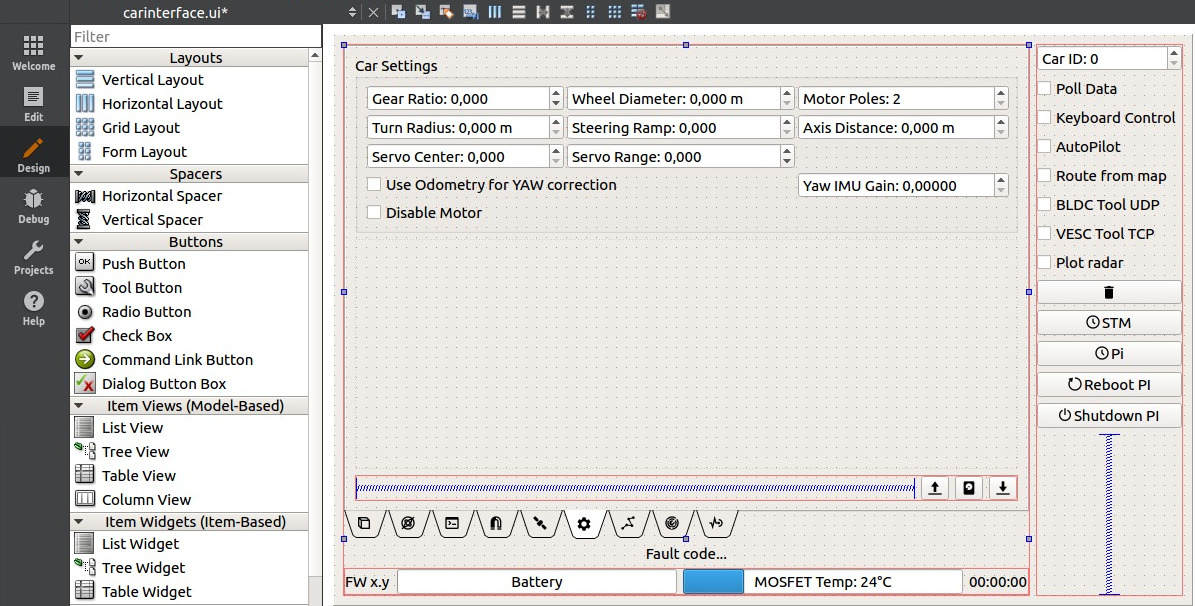
\includegraphics[width=\textwidth]{pictures/GUI_before.jpg}
\end{minipage}
\hfill
\begin{minipage}[b]{0.45\textwidth}
  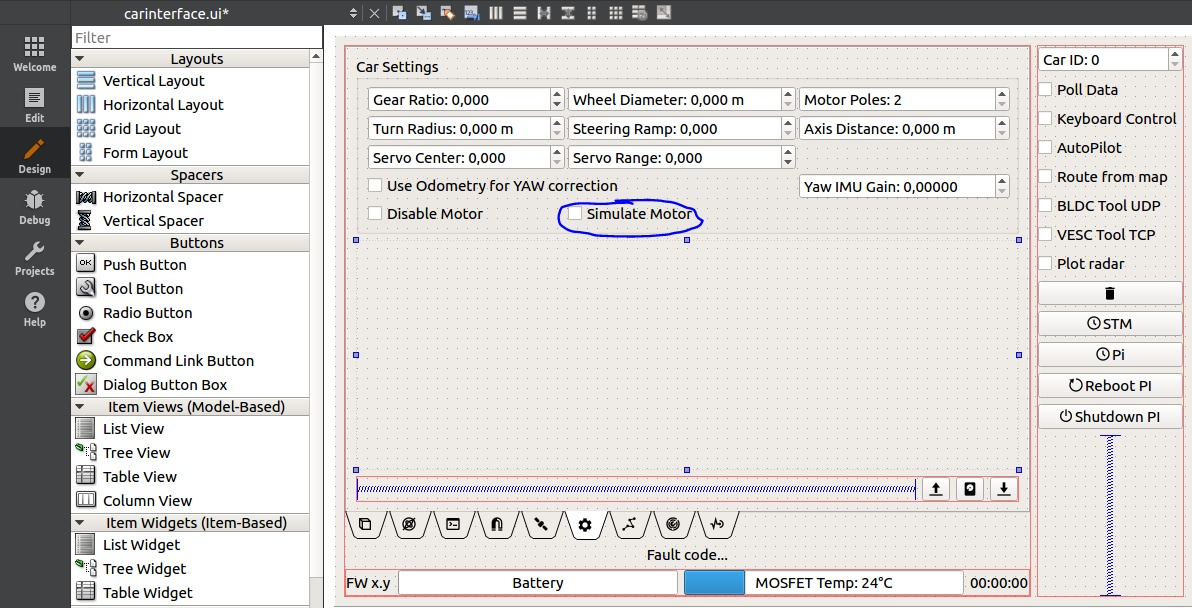
\includegraphics[width=\textwidth]{pictures/GUI_after.jpg}
\end{minipage}

Add a checkbox by dragging one from the list of ``widgets'' to the
left onto the edit area and drop it where you want it to reside.

Click on the newly added checkbox to edit its properties. Change its
name (the objectName field) to:
{\verb!confMiscSimulateMotorBox!}. This is how we will refer to the
checkbox in the rest of the code.

\section{Changes to the RControlStation Code}
The changes up to this point have been purely aesthetic. Some plumbing
is required in order to grab/set the value of the checkbox from/to the
GUI presentation of it.

First we need somewhere to store the value of the checkbox. In
{\verb!datatypes.h!} there is a struct called {\verb!MAIN_CONFIG!}.
It contains a number of common vehicle settings (applicable to both
car and quadracopter) but at the end it contains two vehicle specific
structs, {\verb!MAIN_CONFIG_CAR car!} and {\verb!MAIN_CONFIG_MULTIROTOR mr!}.

\begin{Verbatim}[samepage=true,frame=single,label=Linux/RControlStation/datatypes.h]
// Car configuration
typedef struct {
    // Common vehicle settings
    bool mag_use; // Use the magnetometer
    bool mag_comp; // Should be 0 when capturing samples for the calibration
    float yaw_mag_gain; // Gain for yaw angle from magnetometer (vs gyro)

    // Magnetometer calibration
    float mag_cal_cx;
    /* ... */

    // GPS parameters
    float gps_ant_x; // Antenna offset from vehicle center in X
    /* ... */
    
    // Autopilot parameters
    bool ap_repeat_routes; // Repeat the same route when the end is reached
    /* ... */ 
    
    // Logging
    int log_rate_hz;
    bool log_en;
    char log_name[LOG_NAME_MAX_LEN + 1];
    bool log_en_uart;
    int log_uart_baud;

    MAIN_CONFIG_CAR car;
    MAIN_CONFIG_MULTIROTOR mr;
} MAIN_CONFIG;
\end{Verbatim}

{\verb!MAIN_CONFIG_CAR!} is a good candidate for holding the state that
we are adding as it will be specific for the RC car implementation. 

\begin{Verbatim}[samepage=true,frame=single,label=Linux/RControlStation/datatypes.h]
typedef struct {
  bool yaw_use_odometry; 
  float yaw_imu_gain; 
  bool disable_motor;

  float gear_ratio;
  float wheel_diam;
  float motor_poles;
  float steering_max_angle_rad;
  float steering_center;
  float steering_range;
  float steering_ramp_time; 
  float axis_distance;
} MAIN_CONFIG_CAR;
\end{Verbatim}


\change{} Directly after {\verb!bool disable_motor;!} we add {\verb!bool simulate_motor;!}.



%% typedef struct {
%%   bool yaw_use_odometry; // Use odometry data for yaw angle correction.
%%   float yaw_imu_gain; // Gain for yaw angle from IMU (vs odometry)
%%   bool disable_motor; // Disable motor drive commands to make sure that the motor does not move.

%%   float gear_ratio;
%%   float wheel_diam;
%%   float motor_poles;
%%   float steering_max_angle_rad; // = arctan(axist_distance / turn_radius_at_maximum_steering_angle)
%%   float steering_center;
%%   float steering_range;
%%   float steering_ramp_time; // Ramp time constant for the steering servo in seconds
%%   float axis_distance;
%% } MAIN_CONFIG_CAR;


In {\verb!carinterface.cpp!} there is a function that sets values in a
an instance of {\verb!MAIN_CONFIG!} called {\verb!getConfGui!}.  This
function is called every time the ``write configuration'' button is
pressed in the GUI. 

\begin{Verbatim}[samepage=true,frame=single,label=Linux/RControlStation/carinterface.cpp]
void CarInterface::getConfGui(MAIN_CONFIG &conf)
{
    conf.car.yaw_use_odometry = ui->confOdometryYawBox->isChecked();
    conf.car.yaw_imu_gain = ui->confYawImuGainBox->value();
    conf.car.disable_motor = ui->confMiscDisableMotorBox->isChecked();

    conf.car.gear_ratio = ui->confGearRatioBox->value();
    conf.car.wheel_diam = ui->confWheelDiamBox->value();
    
    /* ... */
    
    ui->confCommonWidget->getConfGui(conf);
}
\end{Verbatim}

\change{} Add code to this function that sets
       {\verb!conf.car.simulate_motor!} to the value of
       {\verb!ui->confMiscSimulateMotorBox->isChecked()!}.


If we take a look at the {\verb!on_confWriteButton_clicked()!}
function (that calls {\verb!getConfGui!}), we see that it will try
to ``set'' (upload to vehicle) the configuration that it read out of
the GUI.

\begin{Verbatim}[samepage=true,frame=single,label=Linux/RControlStation/carinterface.cpp]
void CarInterface::on_confWriteButton_clicked()
{
   /* ... */ 

    if (mPacketInterface) {
        MAIN_CONFIG conf;
        getConfGui(conf);
        ui->confWriteButton->setEnabled(false);
        bool ok = mPacketInterface->setConfiguration(mId, conf, 5);
        ui->confWriteButton->setEnabled(true);

        /* ... */ 
    }
}
\end{Verbatim}

This piece of code hints that we may need to look into the ``packetInterface''
for some further plumbing.

In {\verb!packetinterface.cpp!} there are two functions that need some
amendment to handle the new field in the configuration
data structure. These functions are {\verb!setConfiguration!} and
{\verb!processPacket!}. Here {\verb!processPacket!} deals with the
  ``unpacking'' of received data and {\verb!setConfiguration!}
  produces a packet to send.


\begin{Verbatim}[samepage=true,frame=single,label=Linux/RControlStation/packetinterface.cpp]
void PacketInterface::processPacket(const unsigned char *data, int len)
{
   
  /* ... */
  
        int32_t ind = 0;

        /* ... */
        
        // Car settings
        conf.car.yaw_use_odometry = data[ind++];
        conf.car.yaw_imu_gain = utility::buffer_get_double32_auto(data, &ind);
        conf.car.disable_motor = data[ind++];

        conf.car.gear_ratio = utility::buffer_get_double32_auto(data, &ind);
        conf.car.wheel_diam = utility::buffer_get_double32_auto(data, &ind);
        conf.car.motor_poles = utility::buffer_get_double32_auto(data, &ind);
        
  /* ... */ 
}
\end{Verbatim}

\change{} Directly after
       {\verb!conf.car.disable_motor = data[ind++];!} add
       \\ {\verb!conf.car.simulate_motor = data[ind++];!}.  The order
       of operations in this code change is important as sender and
       receiver need to agree on where different values reside within
       the data package.



A similar (but in the reverse direction) change is needed in the {\verb!setConfiguration!} function.
       
\begin{Verbatim}[samepage=true,frame=single,label=Linux/RControlStation/packetinterface.cpp]
bool PacketInterface::setConfiguration(quint8 id,
                                       MAIN_CONFIG &conf,
                                       int retries)
{
    qint32 send_index = 0;

    /* ... */ 
    
    // Car settings
    mSendBuffer[send_index++] = conf.car.yaw_use_odometry;
    utility::buffer_append_double32_auto(mSendBuffer,
                                         conf.car.yaw_imu_gain,
                                         &send_index);
    mSendBuffer[send_index++] = conf.car.disable_motor;

    /* ... */
    
    return sendPacketAck(mSendBuffer, send_index, retries, 500);
}
\end{Verbatim}

\change{} Here we add {\verb!mSendBuffer[send_index++] = conf.car.simulate_motor;!} directly
after the line referring to {\verb!disable_motor!}.

With these changes we are done in the {\verb!RControlStation!} GUI and
can switch over to working on the embedded side of the story. 

\section{Changes to the RC\_Controller Code}

Before we start implementation of the motor controller simulator -- for real --
some plumbing (mirroring the RControlStation plumbing) is required in
the RC\_Controller code.


Step one is to make room in the data structure that holds the configuration,
on the embedded side, for the new parameter. This resides in the {\verb!datatypes.h!} file,
now in the {\verb!Embedded\RC_Controller!} directory.

Just as before, there is a {\verb!MAIN_CONFIG!} struct that also contains a
{\verb!MAIN_CONFIG_CAR!} field. It is in this {\verb!MAIN_CONFIG_CAR!} struct that we apply our change. 

\begin{Verbatim}[samepage=true,frame=single,label=Embedded/RC\_Controller/datatypes.c]
typedef struct {
	bool yaw_use_odometry; 
	float yaw_imu_gain; 
	bool disable_motor;

	float gear_ratio;
	float wheel_diam;
	float motor_poles;
	float steering_max_angle_rad; 
	float steering_center;
	float steering_range;
	float steering_ramp_time; 
	float axis_distance;
} MAIN_CONFIG_CAR;
\end{Verbatim}

\change Add {\verb!bool simulate_motor;!} directly after {\verb!bool disable_motor;!}.


The file {\verb!conf_general.c!} contains a default configuration. We need to
alter this with the new parameter in mind. 

\begin{Verbatim}[samepage=true,frame=single,label=Embedded/RC\_Controller/conf\_general.c]
void conf_general_get_default_main_config(MAIN_CONFIG *conf) {

        /* ... */ 

	// Default car settings
	conf->car.yaw_use_odometry = false;
	conf->car.yaw_imu_gain = 0.5;
	conf->car.disable_motor = false;

	conf->car.gear_ratio = (1.0 / 3.0) * (21.0 / 37.0);
	conf->car.wheel_diam = 0.12;
	conf->car.motor_poles = 4.0;
	conf->car.steering_max_angle_rad = 0.42041;
	conf->car.steering_center = 0.5;
	conf->car.steering_range = 0.58;
	conf->car.steering_ramp_time = 0.6;
	conf->car.axis_distance = 0.475;

        /* ... */ 
}
\end{Verbatim}

A sensible default setting for {\verb!simulate_motor!} is off. So let's set this
to false.

\change{} Add {\verb!conf->car.simulate_motor = false;!}. 

The file {\verb!conf_general.h!} contains version information for the embedded software.
This should be changed as part of adding new functionality (or fixing bugs). But as the current
version is a moving target I leave this part out of this description.


Now we need to make changes that are similar to the ones we did in
{\verb!packetinterface.cpp!} (in the GUI) to the embedded
software. This functionality is located in {\verb!commands.c!}.  The
function containing the code snippet below is huge! Searching for
``Car Settings'' brings you close to a good place to edit. The {\verb!main_config!}
that the code refers to is a global that resides in {\verb!conf_general.c!}.

\begin{Verbatim}[samepage=true,frame=single,label=Embedded/RC\_Controller/commands.c]
void commands_process_packet(unsigned char *data, unsigned int len,
		void (*func)(unsigned char *data, unsigned int len)) {

  /* ... */
                  
  // Car settings
  main_config.car.yaw_use_odometry = data[ind++];
  main_config.car.yaw_imu_gain = buffer_get_float32_auto(data, &ind);
  main_config.car.disable_motor = data[ind++];

  main_config.car.gear_ratio = buffer_get_float32_auto(data, &ind);
  main_config.car.wheel_diam = buffer_get_float32_auto(data, &ind);
  main_config.car.motor_poles = buffer_get_float32_auto(data, &ind);
  
  /* ... */
  
}
\end{Verbatim}

\change{} Add {\verb!main_config.car.simulate_motor = data[ind++];!} directly after the
line where {\verb!disable_motor!} is set.

The change above is concerned with the reception of configuration
data. A similar change is needed also to transmit. This is handled in the same function
upon reception of a {\verb!GET_MAIN_CONFIG!} command. 

\begin{Verbatim}[samepage=true,frame=single,label=Embedded/RC\_Controller/commands.c]
void commands_process_packet(unsigned char *data, unsigned int len,
		void (*func)(unsigned char *data, unsigned int len)) {

  /* ... */ 
                  
                  
  // Car settings
  m_send_buffer[send_index++] = main_cfg_tmp.car.yaw_use_odometry;
  buffer_append_float32_auto(m_send_buffer,
                            main_cfg_tmp.car.yaw_imu_gain,
                            &send_index);
  m_send_buffer[send_index++] = main_cfg_tmp.car.disable_motor;

  buffer_append_float32_auto(m_send_buffer,
                            main_cfg_tmp.car.gear_ratio,
                            &send_index);
                  
  /* ... */ 
  
}
\end{Verbatim}

\change{} Add
       {\verb!m_send_buffer[send_index++] = main_cfg_tmp.car.simulate_motor;!}
       after the line that handles {\verb!disable_motor!}. Again the
       ordering is of importance.


The plumbing is now done. The GUI and the embedded software can
exchange configurations that include the {\verb!simulate_motor!}
field.  The next step is to implement logic that responds to
{\verb!simulate_motor!} being set on the embedded end and to pretend
to be a motor controller instead of trying to communicate with the
actual motor control board.
       
      
\section{Implementation of the Motor Control Simulator} \label{sec:implementation}

Now, the plan is to implement functionality that pretends to be the
motor controller. To start with we investigate the existing interface
used to talk to the motor controller.

The motor controller interface is defined in the files
{\verb!bldc_interface.c!} and {\verb!bldc_interface.h!} (bldc -
Brushless DC motor).  Below we show a set of functions from the bldc
interface that are used to control the vehicles movement as well as a
function used to signal that we want values from the motor controller.

%\begin{Verbatim}[samepage=true,frame=single,label=Embedded/RC\_Controller/bldc\_interface.c]
%void bldc_interface_init(void(*func)(unsigned char *data, unsigned int len)) {
%	send_func = func;
%}
%\end{Verbatim}

The functions, listed below, all create a ``packet'' consisting of a
command and a value that is then sent to the motor controller.


\begin{Verbatim}[samepage=true,frame=single,label=Embedded/RC\_Controller/bldc\_interface.c]
void bldc_interface_set_duty_cycle(float dutyCycle) {
	int32_t send_index = 0;
	send_buffer[send_index++] = COMM_SET_DUTY;
	buffer_append_float32(send_buffer, dutyCycle, 100000.0, &send_index);
	send_packet_no_fwd(send_buffer, send_index);
}
\end{Verbatim}

Controls engine based on ``dutyCycle'', as a proportion of battery voltage. 


\begin{Verbatim}[samepage=true,frame=single,label=Embedded/RC\_Controller/bldc\_interface.c]
void bldc_interface_set_current(float current) {
	int32_t send_index = 0;
	send_buffer[send_index++] = COMM_SET_CURRENT;
	buffer_append_float32(send_buffer, current, 1000.0, &send_index);
	send_packet_no_fwd(send_buffer, send_index);
}
\end{Verbatim}

This function controls the engine by specifying a current value. 

\begin{Verbatim}[samepage=true,frame=single,label=Embedded/RC\_Controller/bldc\_interface.c]
void bldc_interface_set_current_brake(float current) {
	int32_t send_index = 0;
	send_buffer[send_index++] = COMM_SET_CURRENT_BRAKE;
	buffer_append_float32(send_buffer, current, 1000.0, &send_index);
	send_packet_no_fwd(send_buffer, send_index);
}
\end{Verbatim}

Same as above but only allowed to brake. (TODO: What does this mean? What are the allowed values of ``current''.)

\begin{Verbatim}[samepage=true,frame=single,label=Embedded/RC\_Controller/bldc\_interface.c]
void bldc_interface_set_rpm(int rpm) {
	int32_t send_index = 0;
	send_buffer[send_index++] = COMM_SET_RPM;
	buffer_append_int32(send_buffer, rpm, &send_index);
	send_packet_no_fwd(send_buffer, send_index);
}
\end{Verbatim}

Control engine by specifying an RPM. 

\begin{Verbatim}[samepage=true,frame=single,label=Embedded/RC\_Controller/bldc\_interface.c]
void bldc_interface_set_pos(float pos) {
	int32_t send_index = 0;
	send_buffer[send_index++] = COMM_SET_POS;
	buffer_append_float32(send_buffer, pos, 1000000.0, &send_index);
	send_packet_no_fwd(send_buffer, send_index);
}
\end{Verbatim}

This function (``set\_pos'') is not used!

\begin{Verbatim}[samepage=true,frame=single,label=Embedded/RC\_Controller/bldc\_interface.c]
void bldc_interface_get_values(void) {
	int32_t send_index = 0;
	send_buffer[send_index++] = COMM_GET_VALUES;
	send_packet_no_fwd(send_buffer, send_index);
}
\end{Verbatim}


\subsection{Changes to the BLDC Interface}

We can hijack The functions shown in the previous section and stop them from
sending messages downwards to the lower level motor control. Instead they
can communicate with a thread that maintains a simulated motor state. The
motor simulation thread is implemented in section \ref{sec:simthread}. 


We hijack the interface functions by checking if a function pointer is
non-null. The function pointers we need are defined as follows:

\begin{Verbatim}[samepage=true, frame=single, label=Embedded/RC\_Controller/bldc\_interface.c]
static void(*motor_control_set_func)(motor_control_mode mode,float value) = 0;
static void(*values_requested_func)(void) = 0;
\end{Verbatim}

The first of these function pointers will point a function used to replace the different ``set'' functions in the bldc interface. The \verb!values_requested_func!, on the other hand, is used to hijack the ``get'' function.

The changes to the ``set'' functions and the ``get'' function are all
done in a very similar way. So as an example, here the changes to
{\verb!bldv_interface_set_duty_cycle!} are shown:
\begin{Verbatim}[samepage=true, frame=single, label=Embedded/RC\_Controller/bldc\_interface.c]
void bldc_interface_set_duty_cycle(float dutyCycle) {

        if (motor_control_set_func) {
          motor_control_set_func(MOTOR_CONTROL_DUTY, dutyCycle);
          return;
        }
  
	int32_t send_index = 0;
	send_buffer[send_index++] = COMM_SET_DUTY;
	buffer_append_float32(send_buffer, dutyCycle, 100000.0, &send_index);
	send_packet_no_fwd(send_buffer, send_index);
}  
\end{Verbatim} 

If the function pointer is set to a non-null value, the function is
called with the arguments \verb!MOTOR_CONTROL_DUTY! and
\verb!dutyCycle!. The \verb!MOTOR_CONTROL_DUTY! argument is of an enum
type, that identifies the different modes on control, defined as
follows:

\begin{Verbatim}[samepage=true, frame=single, label=Embedded/RC\_Controller/datatypes.h]
typedef enum {
  MOTOR_CONTROL_DUTY = 0,
  MOTOR_CONTROL_CURRENT,
  MOTOR_CONTROL_CURRENT_BRAKE,
  MOTOR_CONTROL_RPM,
  MOTOR_CONTROL_POS
} motor_control_mode;
\end{Verbatim}


We also add some functions that are used to set the value of the
function pointers: 

\begin{Verbatim}[samepage=true, frame=single, label=Embedded/RC\_Controller/bldc\_interface.c]
void bldc_interface_set_sim_control_function(
       void(*func)(motor_control_mode mode,float value)) {
  motor_control_set_func = func;
}

void bldc_interface_set_sim_values_func(void(*func)(void)) {
  values_requested_func = func;
}
\end{Verbatim}

With these changes in place it is now possible to take over the bldc interface
and pass the values intended for the motor controller to some other system.
In the next section we implement such a system, a motor simulation thread!

\subsection{Implementation of the Motor Simulation Thread}\label{sec:simthread}

The embedded software running on the demoplatform uses
ChibiOS{\footnote{\url{http://www.chibios.org/dokuwiki/doku.php}}. The
  code developed in this section will make use of some ChibiOS
  functionality for thread creation and timing. The few ChibiOS
  functions that are used will be explained as they appear throughout
  the section.

The code we develop in this section goes into a newly created file
called {\verb!motor_sim.c!}. There will also be an associated
{\verb!motor_sim.h!} file containing the interface to using the motor
simulator.

The header file exposes just two functions, one for initialisation and one for seting (or unseting) the motor simulator into running state.

\begin{Verbatim}[samepage=true,frame=single,label=Embedded/RC\_Controller/motor\_sim.h]
#ifndef MOTOR_SIM_H_
#define MOTOR_SIM_H_

#include "datatypes.h"

// Functions
void motor_sim_init(void);
void motor_sim_set_running(bool running);

#endif /* MOTOR_SIM_H_ */
\end{Verbatim}

The {\verb!motor_sim.c!} file starts by including relevant headers. A
few of these headers are ChibiOS related (\verb!ch.h! and
\verb!hal.h!). \verb!bldc_interface.h! is familiar from earlier and
defines the interface to the motor controller. The \verb!utils.h! file
exposes a set of library utility functions used throughout the
demoplatform code.

\begin{Verbatim}[samepage=true,frame=single,label=Embedded/RC\_Controller/motor\_sim.c]
#include <math.h>

#include "motor_sim.h"
#include "ch.h"
#include "hal.h"
#include "bldc_interface.h"
#include "utils.h"
\end{Verbatim}

Next we define some properties of motor (and simulation system), these will be used by
the simulation code later. 

\begin{Verbatim}[samepage=true,frame=single,label=Embedded/RC\_Controller/motor\_sim.c]  
// Settings
#define SIMULATION_TIME_MS 10
#define MOTOR_KV           520.0
#define MOTOR_POLES        4.0
#define INPUT_VOLTAGE      39.0
#define ERPM_PER_SEC       25000.0
#define MAX_CURRENT        80.0
#define TIMEOUT            2.0
\end{Verbatim}

\begin{itemize}
\item \verb!MOTOR_KV! If the engine is spun this many RPM it will generate 1V of ``back-emf''. It can also be seen as an estimate of the number of RPM produced given 1V of an unloaded engine.
\item \verb!MOTOR_POLES! Number of motor poles. 
\item \verb!INPUT_VOLTAGE! The voltage on our simulated battery. 
\item \verb!ERPM_PER_SEC! Maximum change in ``electrical''-RPM per time unit.
  RPM and ERPM are related by $ERPM = RPM*(MOTOR\_POLES/2))$
\item \verb!MAX_CURRENT! Maximum current allowed (amperes).
\item \verb!SIMULATION_TIME_MS! The simulation code is executed every \verb!SIMULATION_TIME_MS!. Sets the simulation period. 
\item \verb!TIMEOUT! Maximum time allowed without interaction with the simulated motor controller.
\end{itemize}

Next we declare a set of variables representing the simulator state.

\begin{Verbatim}[samepage=true,frame=single,label=Embedded/RC\_Controller/motor\_sim.c]
// Private variables
static bool m_is_running;
static mc_values m_values;
static motor_control_mode m_mode;
static float m_mode_value;
static float m_timeout;
\end{Verbatim}

\begin{itemize}
\item \verb!m_is_running! Is set to true when simulation mode is started.
\item \verb!m_values! Will hold simulated motor controller state. The m\verb!c_values! type is located in \verb!datatypes.h! and shown below.
\item \verb!m_mode! Can be one of the following:
  \verb!MOTOR_CONTROL_DUTY!, \verb!MOTOR_CONTROL_CURRENT!,
  \verb!MOTOR_CONTROL_CURRENT_BRAKE!, \verb!MOTOR_CONTROL_RPM!,
  \verb!MOTOR_CONTROL_POS!.
\item \verb!m_mode_value! Is the value communicated through the
  interface. its interpretaion is different depending on
  \verb!m_mode!.
\item \verb!m_timeout! Accumulates time in order to keep track of
    timeouts. Value is reset at every message received from motor
    controller.
\end{itemize}


\begin{Verbatim}[samepage=true,frame=single,label=Embedded/RC\_Controller/datatypes.h]
typedef struct {
	float v_in;
	float temp_mos;
	float temp_motor;
	float current_motor;
	float current_in;
	float id;
	float iq;
	float rpm;
	float duty_now;
	float amp_hours;
	float amp_hours_charged;
	float watt_hours;
	float watt_hours_charged;
    int tachometer;
    int tachometer_abs;
    mc_fault_code fault_code;
} mc_values;
\end{Verbatim}


The following functions are used in the hijacking of the motor
controller interface. 
\begin{Verbatim}[samepage=true,frame=single,label=Embedded/RC\_Controller/motor\_sim.c]
// Private functions
static void motor_control_set(motor_control_mode mode, float value);
static void motor_values_requested(void);
\end{Verbatim}

The motor simulator will be a ChibiOS thread. The following sets up
thread working area (memory for the threads stack and such) and
declares a thread function.

\begin{Verbatim}[samepage=true,frame=single,label=Embedded/RC\_Controller/motor\_sim.c]
// Threads
static THD_WORKING_AREA(sim_thread_wa, 2048);
static THD_FUNCTION(sim_thread, arg);
\end{Verbatim}


Now we are stepping into the actual code of the simulator. The
initialisation function sets default values to simulation state
variables and creates a ChibiOS thread.
\begin{Verbatim}[samepage=true,frame=single,label=Embedded/RC\_Controller/motor\_sim.c]
void motor_sim_init(void) {
	m_is_running = false;
	m_mode = MOTOR_CONTROL_DUTY;
	m_mode_value = 0.0;
	m_timeout = 0.0;
	chThdCreateStatic(sim_thread_wa,
                          sizeof(sim_thread_wa),
                          NORMALPRIO,
                          sim_thread,
                          NULL);
}

\end{Verbatim}

The \verb!motor_sim_set_running! function is part of the interface to
the motor simulator and is run when configuration is set on the
car. if simulation is on, this function configures the motor
controller to pass values to a set of supplied functions in the motor
simulator.

\begin{Verbatim}[samepage=true,frame=single,label=Embedded/RC\_Controller/motor\_sim.c]
void motor_sim_set_running(bool running) {
	m_is_running = running;

	if (m_is_running) {
		bldc_interface_set_sim_control_function(motor_control_set);
		bldc_interface_set_sim_values_func(motor_values_requested);
	} else  {
		bldc_interface_set_sim_control_function(0);
		bldc_interface_set_sim_values_func(0);
	}
}
\end{Verbatim}

Next up is the thread function. This is where the work takes place and
it is a slightly bigger function than what we have seen so far. This
function will be split up and explained in parts.

\begin{Verbatim}[samepage=false,frame=single,label=Embedded/RC\_Controller/motor\_sim.c]
static THD_FUNCTION(sim_thread, arg) {
	(void)arg;

	chRegSetThreadName("MotorSim");

	systime_t iteration_timer = chVTGetSystemTime();
\end{Verbatim}

The \verb!THD_FUNCTION(name, arg)! macro expands into a function
declaration as \verb!void name(void *arg)!, the exact expansion may be
platform dependent.

The first thing \verb!sim_thread! does is to register the name
``MotorSim'' with the ChibiOS thread registry. This is mainly a debug
functionality that provides the ability to enumarate running threads
and their state.

Then we grab an initial value for the iteration timer using
\verb!chVTGetSystemTime()!, this is used later to achieve a simulation
period.

Then the thread enters into an infinite loop. Each iteration of the
loop calculates a new set of \verb!mc_values!, the \verb!m_values!
  value, representing the current state of the motor. Parts of the
  loop body has been broken out and replaced with a C comment, these
  parts are shown individually below.

\begin{Verbatim}[samepage=false,frame=single,label=Embedded/RC\_Controller/motor\_sim.c]        
	for(;;) {
		float dt = (float)SIMULATION_TIME_MS / 1000.0;

		if (m_is_running) {
		        const float rpm_max = INPUT_VOLTAGE *
                                              MOTOR_KV *
                                              (MOTOR_POLES / 2.0);

			switch (m_mode) {
                           /* CASES GO HERE */ 

			default:
				break;
			}

                        /* Friction calculation */

                        /* Update values */

                        /* Consider timeout */
                        

		}

		iteration_timer = chThdSleepUntilWindowed(iteration_timer,
				iteration_timer + MS2ST(SIMULATION_TIME_MS));
	}
}
\end{Verbatim}

At the end of the for loop the thread is put to sleep for enough time
to be restarted again roughly every \verb!SIMULATION_TIME_MS!. the
\verb!dt! value defined at the beginning of the loop represents the
simulation periond in seconds.


Below the different mode cases are listed and explained (to some small
degree). Each of these cases make use of an util function for stepping
a value towards some goal in a specified increment
(\verb!utils_step_towards!).

In the \verb!DUTY! mode, the \verb!m_mode_value! (passed from the interface)
represents a percentage of max potential. In this case the engine will reach an
RPM that is the same percentage of maximum RPM.

\begin{Verbatim}[samepage=true,frame=single,label=Embedded/RC\_Controller/motor\_sim.c]
  case MOTOR_CONTROL_DUTY: {
    float rpm = m_mode_value * rpm_max;
    utils_step_towards(&m_values.rpm,
                       rpm,
                       ERPM_PER_SEC * dt);
  } break;
\end{Verbatim}

In \verb!CURRENT! mode the engine will accelerate towards its maximum
RPM at a rate decided by percentage of current (out of
\verb!MAX_CURRENT!) that is applied.

\begin{Verbatim}[samepage=true,frame=single,label=Embedded/RC\_Controller/motor\_sim.c]
  case MOTOR_CONTROL_CURRENT: {
    utils_step_towards(&m_values.rpm,
                       SIGN(m_mode_value) *
                       rpm_max,
	               ERPM_PER_SEC * dt *
                          (fabsf(m_mode_value) /
                          MAX_CURRENT));
  } break;
\end{Verbatim}

The \verb!CURRENT_BRAKE! mode is very similar to the \verb!CURRENT!
mode above, but the \verb!m_mode_value! is assumed to represent only
braking. (Doesn't braking mean different things if we are moving forward or reversing?) 

\begin{Verbatim}[samepage=true,frame=single,label=Embedded/RC\_Controller/motor\_sim.c]
  case MOTOR_CONTROL_CURRENT_BRAKE: {
    utils_step_towards(&m_values.rpm, 0.0,
		       ERPM_PER_SEC * dt *
                         (fabsf(m_mode_value) /
                         MAX_CURRENT));
  } break;
\end{Verbatim}

When using \verb!RPM! mode the \verb!m_mode_value! represents the target RPM. In this case we step the engine RPM towards \verb!m_mode_value! in \verb!ERPM_PER_SEC! increments. 

\begin{Verbatim}[samepage=true,frame=single,label=Embedded/RC\_Controller/motor\_sim.c]
  case MOTOR_CONTROL_RPM: {
    utils_step_towards(&m_values.rpm,
                       m_mode_value,
                       ERPM_PER_SEC * dt);
  } break;
\end{Verbatim}

The \verb!POS! more of control is not considered... 

\begin{Verbatim}[samepage=true,frame=single,label=Embedded/RC\_Controller/motor\_sim.c]
  case MOTOR_CONTROL_POS: {
    // TODO
  } break;
\end{Verbatim}

That concludes the body of the switch statement within the simulation loop. 


Friction is applied at each timestep consisting of an exponential and a linear component. (TODO: Not sure this code is quite as intended.)
\begin{Verbatim}[samepage=true,frame=single,label=Embedded/RC\_Controller/motor\_sim.c]
  // Friction
  m_values.rpm *= powf(0.9, dt);
  utils_step_towards(&m_values.rpm,
                     0.0,
                     ERPM_PER_SEC * dt * 0.02);
\end{Verbatim}


Now the rest of the \verb!m_values! fields can be computed using the
results computed in the cases listed above.

\begin{Verbatim}[samepage=true,frame=single,label=Embedded/RC\_Controller/motor\_sim.c]
  // Update values
  m_values.tachometer += m_values.rpm /
                         60.0 * dt * 6.0;
  m_values.tachometer_abs += fabsf(m_values.rpm) /
                             60.0 * dt * 6.0;
  m_values.v_in = INPUT_VOLTAGE;
  m_values.duty_now = m_values.rpm / rpm_max;
  m_values.temp_mos = 25.0;
  m_values.temp_motor = 25.0;
  m_values.current_motor = 0.0;
  m_values.current_in = m_values.duty_now *
                        m_values.current_motor;
  m_values.id = 0.0;
  m_values.iq = m_values.current_motor;
  m_values.amp_hours = 0.0;
  m_values.amp_hours_charged = 0.0;
  m_values.watt_hours = 0.0;
  m_values.watt_hours_charged = 0.0;
  m_values.fault_code = FAULT_CODE_NONE;
\end{Verbatim}

If timout happens (no interaction with the motor controller in a given inteval) we
apply a breaking force on the motor.

\begin{Verbatim}[samepage=true,frame=single,label=Embedded/RC\_Controller/motor\_sim.c]                        
  // Timeout
  m_timeout += dt;
  if (m_timeout > TIMEOUT) {
    m_mode = MOTOR_CONTROL_CURRENT_BRAKE;
    m_mode_value = 10.0;
  }
\end{Verbatim}                        

With the above addition to the simulation loop, it is done! Following
are implementations of the two functions that form the exported
interface of the motor simulation code.


\begin{Verbatim}[samepage=true,frame=single,label=Embedded/RC\_Controller/motor\_sim.c]
static void motor_control_set(motor_control_mode mode, float value) {
	m_mode = mode;
	m_mode_value = value;
	m_timeout = 0.0;
}
\end{Verbatim} 

\begin{Verbatim}[samepage=true,frame=single,label=Embedded/RC\_Controller/motor\_sim.c]
static void motor_values_requested(void) {
	send_values_to_receiver(&m_values);
}
\end{Verbatim}


\subsection{Starting the Motor Simulation Thread}

All pieces are in place. With some small tweaks to the \verb!main!
  function it will all be done. All that is needed here is to run
  \verb!motor_sim_init! at a suitable place and also to set the
  simulator into running state in case that is what the configuration
  signals.

\begin{Verbatim}[samepage=true,frame=single,label=Embedded/RC\_Controller/main.c]
int main(void) {
	halInit();
	chSysInit();

	led_init();
	ext_cb_init();

#if MAIN_MODE == MAIN_MODE_CAR
	conf_general_init();
        /* ... */
	log_init();
	motor_sim_init();
        /* ... */
#endif

#if MAIN_MODE == MAIN_MODE_MULTIROTOR
        /* ... */
#endif

	comm_usb_init();
	comm_cc2520_init();
	comm_cc1120_init();
	commands_init();

#if MAIN_MODE_IS_VEHICLE
	commands_set_send_func(comm_cc2520_send_buffer);
#endif

#if UBLOX_EN
	ublox_init();
#endif

#if MAIN_MODE == MAIN_MODE_CAR
	motor_sim_set_running(main_config.car.simulate_motor);
#endif

	timeout_configure(2000, 20.0);
        /* ... */
	log_set_uart(main_config.log_en_uart, main_config.log_uart_baud);

	for(;;) {
		chThdSleepMilliseconds(2);
		packet_timerfunc();
	}
}
\end{Verbatim}

The following should also be added to \verb!commands.c! in order to
respond to correctly in relation to configuration changes.

\begin{Verbatim}[samepage=true,frame=single,label=Embedded/RC\_Controller/commands.c]
#if MAIN_MODE == MAIN_MODE_CAR
motor_sim_set_running(main_config.car.simulate_motor);
#endif
\end{Verbatim}

Last, a default state for \verb!simulate_motor! is set in \verb!conf_general.c!.

\begin{Verbatim}[samepage=true,frame=single,label=Embedded/RC\_Controller/conf\_general.c]
conf->car.simulate_motor = false;
\end{Verbatim}

%% \begin{Verbatim}[samepage=true,frame=single,label=Embedded/RC\_Controller/bldc\_interface.c]

%% \end{Verbatim}

%% \begin{Verbatim}[samepage=true,frame=single,label=Embedded/RC\_Controller/bldc\_interface.c]

%% \end{Verbatim}

%% \begin{Verbatim}[samepage=true,frame=single,label=Embedded/RC\_Controller/bldc\_interface.c]

%% \end{Verbatim}

%% \begin{Verbatim}[samepage=true,frame=single,label=Embedded/RC\_Controller/bldc\_interface.c]

%% \end{Verbatim}

%% \begin{Verbatim}[samepage=true,frame=single,label=Embedded/RC\_Controller/bldc\_interface.c]

%% \end{Verbatim}

%% \begin{Verbatim}[samepage=true,frame=single,label=Embedded/RC\_Controller/bldc\_interface.c]

%% \end{Verbatim}






%\thispagestyle{fancy}

% \begin{abstract}
% \end{abstract}


%% \let\oldbibliography\thebibliography
%% \renewcommand{\thebibliography}[1]{%
%%   \oldbibliography{#1}%
%%   \setlength{\itemsep}{1pt}%
%% }

%% {\small
%% % \vspace{-40mm}
%% %\bibliographystyle{abbrvnat}
%% %\bibliographystyle{plain}
%% \bibliographystyle{abbrv}
%% \bibliography{../VR2016/refs}
%% % \bibliography{./refs}
%% }

\end{document}
